\chapter{Introduction to Model Building} 
\label{chap:mod}

{\it All models are wrong, but some are useful.}---George
Box\footnote{George Box (1919-) is a famous statistician, with several
statistical procedures named after him.}

{\it [Mathematical models] should be made as simple as possible, but not
simpler.}---Albert Einstein\footnote{The reader is undoubtedly aware of
Einstein's (1879-1955) famous theories of relativity, but may not know
his connections to probability theory.  His work on {\bf Brownian
motion}, which describes the path of a molecule as it is bombarded by
others, is probabilistic in nature, and later developed into a major 
branch of probability theory.  Einstein was also a pioneer in quantum
mechanics, which is probabilistic as well.  At one point, he doubted the
validity of quantum theory, and made his famous remark, ``God does not
play dice with the universe.''}

{\it Beware of geeks bearing formulas.}---Warrent Buffett, 2009, on the
role of ``quants'' (Wall Street analysts who form probabilistic models
for currency, bonds etc.) in the 2008 financial collapse.

\bigskip

The above quote by Box says it all.  Consider for example the family of
normal distributions.  In real life, random variables are bounded---no
person's height is negative or greater than 500 inches---and are
inherently discrete, due to the finite precision of our measuring
instruments.  Thus, technically, no random variable in practice
can have an exact normal distribution.  Yet the assumption of normality
pervades statistics, and has been enormously successful, provided one
understands its approximate nature.  

The situation is similar to that of physics.  Paraphrasing Box, we might
say ``Tthe physical models used when engineers design an airplane wing
are all wrong---but they are useful.''  We know that in many analyses of
bodies in motion, we can neglect the effect of air resistance.  But we
also know that in some situations one must include that factor in our
model.

So, the field of probability and statistics is fundamentally about {\it
modeling}.  The field is extremely useful, provided the user understands
the modeling issues well.  For this reason, this book contains this
separate chapter on modeling issues.

\section{``Desperate for Data''}
\label{dfd}

Suppose we have the samples of men's and women's heights, $X_1,...,X_n$
and $Y_1,...,Y_n$.  Assume for simplicity that the variance of height is
the same for each gender, $\sigma^2$.  The means of the two populations
are designated by $\mu_1$ and $\mu_2$.

Say we wish to guess the height of a new person who we know to be a man
but for whom we know nothing else.  We do not see him, etc.

\subsection{Known Distribution}
\label{known}

Suppose for just a moment that we actually know the distribution of X,
i.e. the {\it population} distribution of male heights.  What would be
the best constant g to use as our guess for a person about whom we know
nothing other than gender?

Well, we might borrow from Section \ref{bv} and use mean squared error, 

\begin{equation}
E[(g-X)^2]
\end{equation}

as our criterion of goodness of guessing.  But we already know what the
best g is, from Section \ref{gofc}:  The best g is $\mu_1$.  Our best
guess for this unseen man's height is the mean height of all men in the
population.

\subsection{Estimated Mean}

Of course, we don't know $\mu_1$, but we can do the next-best thing,
i.e. use an estimate of it from our sample.

The natural choice for that estimator would be

\begin{equation}
T_1 = \overline{X},
\end{equation}

the mean height of men in our sample.

But what if n is really small, say n = 5?  That's awfully small.  We may
wish to consider adding the women's heights to our estimate, in order to
get a larger sample.  Then we would estimate $\mu_1$ by

\begin{equation}
T_2 = \frac{\overline{X}+\overline{Y}}{2}, 
\end{equation}

It may at first seem obvious that $T_1$ is the better estimator.  Women
tend to be shorter, after all, so pooling the data from the two genders
would induce a bias.  On the other hand, we found in Section \ref{bv}
that for any estimator,

\begin{equation}
\textrm{MSE = variance of the estimator} + \textrm{bias of the
estimator} ^2
\end{equation}

In other words, {\it some amount of bias may be tolerable}, if it will
buy us a subtantial reduction in variance.  After all, women are not
that much shorter than men, so the bias might not be too bad.
Meanwhile, the pooled estimate should have lower variance, as it is
based on 2n observations instead of n; (\ref{barmean}) indicates that.

Before continuing, note first that $T_2$ is based on a simpler model
than is $T_1$, as $T_2$ ignores gender.  We thus refer to $T_1$ as being
based on the more complex model.

Which one is better?  The answer will need a criterion for
goodness of estimation, which we will take to be mean squared error,
MSE.  So, the question becomes, which has the smaller MSE, $T_1$ or
$T_2$?  In other words:

\begin{quote}
Which is smaller, $E[(T_1 - \mu_1)^2]$ or $E[(T_2 - \mu_1)^2]$?
\end{quote}

\subsection{The Bias/Variance Tradeoff}
\label{biasvartradeoff}

We could calculate MSE from scratch, but it would probably be better to
make use of the work we already went through, producing (\ref{vb2}).
This is especially true in that we know a lot about variance of sample
means, and we will take this route.

So, let's find the biases of the two estimators.

\begin{itemize}

\item $T_1$

$T_1$ is unbiased, from (\ref{barmean}).   So,

\begin{quote}
bias of $T_1 = 0$ 
\end{quote}

\item $T_2$ 

\begin{eqnarray}
E(T_2) &=& E(0.5 \overline{X} + 0.5 \overline{Y}) ~~ (\textrm{definition}) \\
&=& 0.5 E\overline{X} + 0.5 E\overline{Y} ~~ (\textrm{linearity of E()}) \\
&=& 0.5 \mu_1 + 0.5 \mu_2 ~~ [\textrm{from (\ref{barmean})}] 
\end{eqnarray}

So, 

\begin{quote}
bias of $T_2 = (0.5 \mu_1 + 0.5 \mu_2) - \mu_1$
\end{quote}

\end{itemize}

On the other hand, $T_2$ has a smaller variance than $T_1$:  

\begin{itemize}

\item $T_1$ 

Recalling
(\ref{oneovernpopvar}), we have

\begin{equation}
Var(T_1) = \frac{\sigma^2}{n}
\end{equation}

\item $T_2$ 

\begin{eqnarray}
Var(T_2) &=& Var(0.5 \overline{X} + 0.5 \overline{Y}) \\ 
&=& 0.5^2 Var(\overline{X}) + 0.5^2 Var(\overline{Y}) ~~ (\textrm{properties of
Var()}) \\
&=& 2 \cdot 0.25 \cdot \frac{\sigma^2}{n} ~~ [\textrm{from
\ref{oneovernpopvar}}] \label{t2var} \\
&=& \frac{\sigma^2}{2n}
\end{eqnarray}

\end{itemize}

% Once again, think of the notebook analogy.  Each line of the notebook
% would correspond to a sample of n men and women.  Those 2n heights would
% be listed within the row, and there would be columns for $T_1$ and
% $T_2$.  Then for instance $\mu_1$ would be the long-run average of $T_1$
% in its column of the notebook, while (\ref{t2var}) would be the long-run
% variance of $T_2$ in its column. 

% \checkpoint

These findings are highly instructive.  You might at first think that
``of course'' $T_1$ would be the better predictor than $T_2$.  But for a
small sample size, the smaller (actually 0) bias of $T_1$ is not enough
to counteract its larger variance.  $T_2$ is biased, yes, but it is
based on double the sample size and thus has half the variance.

In light of (\ref{vb2}), we see that $T_1$, the ``true'' predictor, may
not necessarily be the better of the two predictors.  Granted, it has no 
bias whereas $T_2$ does have a bias, but the latter has a smaller
variance.

So, under what circumstances will $T_1$ be better than $T_2$?  Let's
answer this by using (\ref{mseformula}):

\begin{equation}
\label{t1}
MSE(T_1) = \frac{\sigma^2}{n} + 0^2 = \frac{\sigma^2}{n} 
\end{equation}

\begin{equation}
\label{t2}
MSE(T_2) = \frac{\sigma^2}{2n} + \left ( \frac{\mu_1+\mu_2}{2} - \mu_1
\right )^2 = \frac{\sigma^2}{2n} + \left ( \frac{\mu_2-\mu_1}{2} \right
)^2
\end{equation}

$T_1$ is a better predictor than $T_2$ if (\ref{t1}) is smaller than
(\ref{t2}), which is true if

\begin{equation}
\label{betteriff}
\left ( \frac{\mu_2-\mu_1}{2} \right)^2 >
\frac{\sigma^2}{2n}
\end{equation}

Granted, we don't know the values of the $\mu_1$ and $\sigma^2$, so in a
real situation, we won't really know whether to use $T_1$ or $T_2$.  But
the above analysis makes the point that under some circumstances, it
really is better to pool the data in spite of bias.

% Of course, we could also use our sample to estimate the $\mu_1$ and
% $\sigma^2$, and then plug in to (\ref{betteriff}).  We would then
% use either $T_1$ or $T_2$ on that basis.  This might work well; we could
% investigate via simulation.

\subsection{Implications}
\label{biasvvariance}

So you can see that $T_1$ is better only if either

\begin{itemize}

\item n is large enough, or

\item the difference in population mean heights between men and women is
large enough, or

\item there is not much variation within each population, e.g. most men
have very similar heights

\end{itemize}

Since that third item, small within-population variance, is rarely seen,
let's concentrate on the first two items.  The big revelation here is
that:

\begin{quote}
A more complex model is more accurate than a simpler one only if either 

\begin{itemize}

\item we have enough data to support it, or

\item the complex model is sufficiently different from the simpler one

\end{itemize}

\end{quote}

{\bf In height/gender example above, if n is too small, we are ``desperate
for data,'' and thus make use of the female data to augment our male
data.}  Though women tend to be shorter than men, the bias that results
from that augmentation is offset by the reduction in estimator variance
that we get.  But if n is large enough, the variance will be small in
either model, so when we go to the more complex model, the advantage
gained by reducing the bias will more than compensate for the increase
in variance. 

{\bf THIS IS AN ABSOLUTELY FUNDAMENTAL NOTION IN STATISTICS.}

% \checkpoint

This was a very simple example, but you can see that in complex
settings, fitting too rich a model can result in very high MSEs for the
estimates.  In essence, everything becomes noise.  (Some people have
cleverly coined the term {\bf noise mining}, a play on the term {\bf
data mining}.)  This is the famous {\bf overfitting} problem.

In our unit on statistical relations, Chapter \ref{chap:linreg}, we will show
the results of a scary experiment done at the Wharton School, the
University of Pennsylvania's business school.  The researchers
deliberately added fake data to a prediction equation, and standard
statistical software identified it as ``significant''!  This is partly a
problem with the word itself, as we saw in Section \ref{whatswrong}, but
also a problem of using far too complex a model, as will be seen in that
future unit.

Note that of course (\ref{betteriff}) contains several unknown
population quantities.  I derived it here merely to establish a
\underline{principle}, namely that a more complex model may perform more
poorly under some circumstances.

It would be possible, though, to make (\ref{betteriff}) into a practical
decision tool, by estimating the unknown quantities, e.g. replacing
$\mu_1$ by $\overline{X}$.  This then creates possible problems with
confidence intervals, whose derivation did not include this extra decision
step.  Such estimators, termed {\bf adaptive}, are beyond the scope of
this book.

\section{Assessing ``Goodness of Fit'' of a Model}
\label{gof}

Our example in Section \ref{gammamle} concerned how to estimate the
parameters of a gamma distribution, given a sample from the
distribution.  But that assumed that we had already decided that the
gamma model was reasonable in our application.  Here we will be
concerned with how we might come to such decisions.

Assume we have a random sample $X_1,...,X_n$ from a distribution having
density $f_X$.  To keep things simple, let's suppose we are considering
an exponential model.

\subsection{The Chi-Square Goodness of Fit Test}
\label{chisqgof}

The classic way to do this would be the {\bf Chi-Square Goodness of Fit
Test}.  We would set

\begin{equation}
H_0:  f_X ~ \textrm{is a member of the exponential parametric family}
\end{equation}

This would involve partitioning $(0,\infty)$ into k intervals
$(s_{i-1},s_i)$ of our choice, and setting 

\begin{equation}
N_i =  \textrm{number of } X_i \textrm{ in } (s_{i-1},s_i) 
\end{equation}

We would then find the Maximum Likelihood Estimate (MLE) of $\lambda$,
on the assumption that the distribution of X really is exponential.  The
MLE turns out to be the reciprocal of the sample mean, i.e. 

\begin{equation}
\widehat{\lambda} = 1/\overline{X}
\end{equation}

This would be considered the parameter of the ``best-fitting''
exponential density for our data.  We would then estimate the
probabilities

\begin{equation}
p_i = P[X \epsilon (s_{i-1},s_i)] = 
e^{-\lambda s_{i-1}} -
e^{-\lambda s_{i}}, ~ i = 1,...,k.
\end{equation}

by

\begin{equation}
\widehat{p_i} = 
e^{-\widehat{\lambda} s_{i-1}} -
e^{-\widehat{\lambda} s_{i}}, ~ i = 1,...,k.
\end{equation}

Note that $N_i$ has a binomial distribution, with n trials and success
probability $p_i$.  Using this, the expected value of $EN_i$ is
estimated to be

\begin{equation}
\nu_i = n(
e^{-\widehat{\lambda} s_{i-1}} -
e^{-\widehat{\lambda} s_{i}}), ~ i = 1,...,k.
\end{equation}

Our test statistic would then be

\begin{equation}
Q = \sum_{i=1}^k \frac{(N_i-v_i)^2}{v_i}
\end{equation}

where $v_i$ is the expected value of $N_i$ under the assumption of
``exponentialness.''  It can be shown that Q is approximately chi-square
distributed with k-2 degrees of freedom.\footnote{We have k intervals,
but the $N_i$ must sum to n, so there are only k-1 free values.  We then
subtract one more degree of freedom, having estimated the parameter
$\lambda$.}  Note that only large values of Q should be suspicious, i.e.
should lead us to reject $H_0$; if Q is small, it indicates a good fit.
If Q were large enough to be a ``rare event,'' say larger than
$\chi_{0.95,k-2}$, we would decide NOT to use the exponential model;
otherwise, we would use it.

{\bf Hopefully the reader has immediately recognized the problem here.}
If we have a large sample, this procedure will pounce on tiny deviations
from the exponential distribution, and we would decide not to use the
exponential model---even if those deviations were quite minor.  Again,
no model is 100\% correct, and thus a goodness of fit test will
eventually tell us not to use {\it any} model at all.

% \checkpoint

\subsection{Kolmogorov-Smirnov Confidence Bands}
\label{kolsmi}

Again consider the problem above, in which we were assessing the fit of
a exponential model.  In line with our major point that confidence
intervals are far superior to hypothesis tests, we now present {\bf
Kolmogorov-Smirnov confidence bands}, which work as follows.

Since this method relies on cdfs, recall  
notion of the {\bf empirical distribution function} (ecdf), Section
\ref{ecdfsec}.
It is a sample estimate of a cdf, defined to be the proportion
of $X_i$ that are below t in the sample.  Graphically, $\widehat{F}_X$
is a step function, with jumps at the values of the $X_i$.

What Kolmogorov-Smirnov does is form a {\bf confidence band} around the
empirical cdf of a sample.  The basis for this is that the distribution
of

\begin{equation}
\label{definem}
M = \max_{-\infty < t \infty} |\widehat{F}_X(t) - F_X(t)|
\end{equation}

{\bf is the same for all distributions having a density}.  This 
fact (whose proof is related to the general method for simulating random
variables having a given density, in Section \ref{genrannumgen})
tells us that, without knowing anything about the distribution of
X, we can be sure that M has the same distribution.  And it turns out
that

\begin{equation}
\label{m95}
F_M(1.358 n^{-1/2}) \approx 0.95
\end{equation}

Define ``upper'' and ``lower'' functions

\begin{equation}
U(t) = \widehat{F}_X(t) + 1.358 n^{-1/2}, ~~
L(t) = \widehat{F}_X(t) - 1.358 n^{-1/2}
\end{equation}

So, what (\ref{definem}) and (\ref{m95}) tell us is

\begin{equation}
0.95 \approx P \left (\textrm{the curve } F_X \textrm{ is entirely between U
and L} \right ) 
\end{equation}

So, the pair of curves, (L(t), U(t)) is called a a {\bf 95\% confidence
band} for $F_X$. 

Now suppose we wish to see how well, say, the gamma distribution family
fits our application.  If the band is very wide, we know we really don't
have enough data to decide much about the distribution of X.  But if the
band is narrow but some member of the family is in the band or is close
to it, we would probably decide that the model is a good one.  Once
again, we should NOT pounce on tiny deviations from the model.

Warning:  The Kolmogorov-Smirnov procedure available in
the R language performs only a hypothesis test, rather than forming a
confidence band.  In other words, it simply checks to see whether a
member of the family falls within the band.  This is not what we want,
because we may be perfectly happy if a member is only {\it near} the
band.

% \checkpoint

\subsection{Less Formal Methods}

Of course, another way, this one less formal, of assessing data for
suitability for some model is to plot the data in a histogram or
something of that nature.  In this section, let's explore using ecdfs
for this.  We can plot the ecdf against a fitted model.

Let's try this with the baseball player data (Section \ref{baseball0}).
Here is the code:

\begin{lstlisting}
> library(ggplot2)
> p <- ggplot(bb,aes(Age))
> p + stat_ecdf()  # plot ecdf 
# define a function for the cdf of a fitted normal distribution 
> ncdf <- function(t) pnorm(t,mean=mean(bb$Age),sd=sd(bb$Age))
> p + stat_ecdf() + stat_function(fun=ncdf)
\end{lstlisting}

The resulting plot is in Figure \ref{ecdfpnorm}.  The fitted curve, in
red, is higher than the ecdf on the low end, i.e. age in the early 20s.
In other words, modeling age as normally distributed in the player
population overestimated the number of 20-somethings.  It also
overestimates the number in the late 30s.  But overall, not a bad
approximation.\footnote{Don't confuse this with the Central Limit
Theorem.  Here we are modeling the population itself has having a normal
distribution, not sample means from it.}

\begin{figure}[tb]
\vskip 0.5in
\centerline{
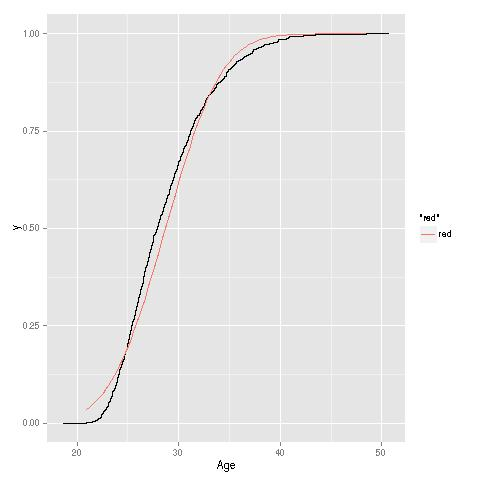
\includegraphics[width=4.5in]{BaseballAge.jpg} 
}
\caption{Ecdf and fitted cdf}
\label{ecdfpnorm}
\end{figure}

% \section{Bias Vs. Variance---Again}
% \label{bvagain}
% 
% In our unit on estimation, Section \ref{nonpardensest}, we saw a classic
% tradeoff in histogram- and kernel-based density estimators.  With
% histograms, for instance, the wider bin width produces a graph which is
% smoother, but possibly {\it too} smooth, i.e. with less oscillation than
% the true population curve has.  The same problem occurs with larger
% values of h in the kernel case.
% 
% This is actually yet another example of the bias/variance tradeoff,
% discussed in above and, as mentioned, {\bf ONE OF THE MOST RECURRING
% NOTIONS IN STATISTICS}.  A large bin width, or a large value of h,
% produces more bias.  In general, the large the bin width or h, the
% further $E[\widehat{f}_R(t)$ is from the true value of $f_R(t)$.  This
% occurs because we are making use of points which are not so near t, and
% thus at which the density height is different from that of $f_R(t)$.  On
% the other hand, because we are making use of more points,
% $Var[\widehat{f}_r(t)]$ will be smaller.
% 
% \checkpoint

Of course, we could do the same with densities.  But that would meaning
choose bin width, bandwidth, number of nearest neighbors or something
like that.  {\bf BUT THERE IS NO GOOD WAY TO CHOOSE THE BIN WIDTH OR h}.
Even though there is a lot of theory to suggest how to choose the bin
width or h, no method is foolproof.  This is made even worse by the fact
that the theory generally has a goal of minimizing {\it integrated} mean
squared error,

\begin{equation}
\int_{-\infty}^{\infty} E \left [ \left ( \widehat{f}_R(t) - f_R(t) \right
)^2 \right ] ~ dt
\end{equation}

rather than, say, the mean squared error at a particular point of
interest, v:

\begin{equation}
E \left [ \left ( \widehat{f}_R(t) - f_R(t) \right)^2 \right ] 
\end{equation}

\section{Robustness}

Traditionally, the term {\it robust} in statistics has meant resilience
to violations in assumptions.  For example, in Section \ref{studentt},
we presented Student-t, a method for finding exact confidence intervals
for means, assuming normally-distributed populations.  But as noted at
the outset of this chapter, no population in the real world has an exact
normal distribution.  The question at hand (which we will address below)
is, does the Student-t method still give approximately correct results
if the sample population is not normal?  If so, we say that Student-t is
{\bf robust} to the normality assumption.

Later, there was quite a lot of interest among statisticians in
estimation procedures that do well even if there are {\bf outliers} 
in the data, i.e. erroneous observations that are in the fringes of the
sample.  Such procedures are said to be robust to outliers.

Our interest here is on robustness to assumptions.  Let us first
consider the Student-t example.  As discussed in Section \ref{studentt},
the main statistic here is

\begin{equation}
T = \frac{\bar{X}-\mu}{s/\sqrt{n}}
\end{equation}

where $\mu$ is the population mean and $s$ is the unbiased version of
the sample variance:

\begin{equation}
s = \sqrt{\frac{\sum_{i=1}^n (X_i-\bar{X})^2}{n-1}}
\end{equation}

The distribution of $T$, under the assumption of a normal population,
has been tabulated, and tables for it appear in virtually every textbook
on statistics.  But what if the population is not normal, as is
inevitably the case?

The answer is that it doesn't matter.  For large n, even for samples
having, say, n = 20, the distribution of $T$ is close to N(0,1) by the
Central Limit Theorem regardless of whether the population is normal.

By contrast, consider the classic procedure for performing hypothesis
tests and forming confidence intervals for a population variance
$\sigma^2$, which relies on the statistic

\begin{equation}
K = \frac{(n-1)s^2}{\sigma^2}
\end{equation}

where again $s^2$ is the unbiased version of the sample variance.
If the sampled population is normal, then $K$ can be shown to have a
chi-square distribution with n-1 degrees of freedom.  This then sets up
the tests or intervals.  However, it has been shown that these
procedures are not robust to the assumption of a normal population.
See {\it The Analysis of Variance: Fixed, Random, and Mixed Models},
by Hardeo Sahai and Mohammed I. Ageel, Springer, 2000, and the earlier
references they cite, especially the pioneering work of Scheffe'.

\section{Real Populations and Conceptual Populations}

In our example in Section \ref{davisweights}, we were sampling from a
real population.  However, in many, probably most applications of
statistics, either the population or the sampling is more conceptual.

Consider an experiment we will discuss in Section \ref{examples},  in
which we compare the programmability of three scripting languages.  (You
need not read ahead.)  We divide our programmers into three groups, and
assign each group to program in one of the languages.  We then compare
how long it took the three groups to finish writing and debugging the
code, and so on.

We think of our programmers as being a random sample from the population
of all programmers, but that is probably an idealization.  We probably
did NOT choose our programmers randomly; we just used whoever we had
available.  But we can think of them as a ``random sample'' from the
rather conceptual ``population'' of all programmers who {\it might} work
at this company.\footnote{You're probably wondering why we haven't
discussed other factors, such as differing levels of experience among
the programmers.  This will be dealt with in our unit on regression
analysis, Chapter \ref{chap:linreg}.}

% And what about the raffle example we'll introduce in Section
% \ref{raffle}?  (Again, you need not read the details there now.)
% Certainly we can imagine various kinds of randomness that contribute
% to
% the numbers people get on their raffle tickets.  Maybe, for instance,
% you were in a traffic jam on the way to the the place where you bought
% the ticket, so you bought it a little later than you might have and
% thus
% got a higher number.  But I've always emphasized the notion of a
% repeatable experiment in these notes.  How can that happen here?  You
% could imagine, for instance, the raffle chair suddenly losing all the
% tickets, and asking everyone to draw again, resulting in different
% ticket numbers.  Or you can imagine the ``population'' of all raffles
% that you might submit to which have the same value of c.

You can see from this that if one chooses to apply statistics
carefully---which you absolutely should do---there sometimes are some
knotty problems of interpretation to think about.


\startproblemset

\oneproblem
In our example in Section \ref{dfd}, assume $\mu_1 = 70, \mu_2= 66,
\sigma = 4$ and the distribution of height is normal in the two
populations.  Suppose we are predicting the height of a man who, unknown
to us, has height 68.  We hope to guess within two inches.  Find $P(|T_1
- 68|) < 2$ and $P(|T_2 - 68|) < 2$ for various values of n.

\oneproblem
In Chapter \ref{chap:simultaninfer} we discuss {\it simultaneous inference},
the forming of confidence intervals whose joint confidence level was
95\% or some other target value.  The Kolmogorov-Smirnov confidence band
in Section \ref{kolsmi} allows us to computer infinitely many confidence
intervals for $F_X(t)$ at different values of t, at a ``price'' of only
1.358.  Still, if we are just estimating $F_X(t)$ at a single value of
t, an individual confidence interval using (\ref{propci}) would be
narrower than that given to us by Kolmogorov-Smirnov.  Compare the
widths of these two intervals in a situation in which the true value of
$F_X(t) = 0.4$.

\oneproblem
Say we have a random sample $X_1,...,X_n$ from a population
with mean $\mu$ and variance $\sigma^2$.  The usual estimator of $\mu$
is the sample mean $\bar{X}$, but here we will use what is called a {\it
shrinkage estimator}:  Our estimate of $\mu$ will be $0.9 \bar{X}$.
Find the mean squared error of this estimator, and give an inequality
(you don't have to algebraically simplify it) that shows under what
circumstances $0.9 \bar{X}$ is better than $\bar{X}$.  (Strong advice:
Do NOT ``reinvent the wheel.''  Make use of what we have already
derived.)

